% Options for packages loaded elsewhere
\PassOptionsToPackage{unicode}{hyperref}
\PassOptionsToPackage{hyphens}{url}
\documentclass[
]{article}
\usepackage{xcolor}
\usepackage{amsmath,amssymb}
\setcounter{secnumdepth}{-\maxdimen} % remove section numbering
\usepackage{iftex}
\ifPDFTeX
  \usepackage[T1]{fontenc}
  \usepackage[utf8]{inputenc}
  \usepackage{textcomp} % provide euro and other symbols
\else % if luatex or xetex
  \usepackage{unicode-math} % this also loads fontspec
  \defaultfontfeatures{Scale=MatchLowercase}
  \defaultfontfeatures[\rmfamily]{Ligatures=TeX,Scale=1}
\fi
\usepackage{lmodern}
\ifPDFTeX\else
  % xetex/luatex font selection
\fi
% Use upquote if available, for straight quotes in verbatim environments
\IfFileExists{upquote.sty}{\usepackage{upquote}}{}
\IfFileExists{microtype.sty}{% use microtype if available
  \usepackage[]{microtype}
  \UseMicrotypeSet[protrusion]{basicmath} % disable protrusion for tt fonts
}{}
\makeatletter
\@ifundefined{KOMAClassName}{% if non-KOMA class
  \IfFileExists{parskip.sty}{%
    \usepackage{parskip}
  }{% else
    \setlength{\parindent}{0pt}
    \setlength{\parskip}{6pt plus 2pt minus 1pt}}
}{% if KOMA class
  \KOMAoptions{parskip=half}}
\makeatother
\usepackage{longtable,booktabs,array}
\newcounter{none} % for unnumbered tables
\usepackage{calc} % for calculating minipage widths
% Correct order of tables after \paragraph or \subparagraph
\usepackage{etoolbox}
\makeatletter
\patchcmd\longtable{\par}{\if@noskipsec\mbox{}\fi\par}{}{}
\makeatother
% Allow footnotes in longtable head/foot
\IfFileExists{footnotehyper.sty}{\usepackage{footnotehyper}}{\usepackage{footnote}}
\makesavenoteenv{longtable}
\usepackage{graphicx}
\makeatletter
\newsavebox\pandoc@box
\newcommand*\pandocbounded[1]{% scales image to fit in text height/width
  \sbox\pandoc@box{#1}%
  \Gscale@div\@tempa{\textheight}{\dimexpr\ht\pandoc@box+\dp\pandoc@box\relax}%
  \Gscale@div\@tempb{\linewidth}{\wd\pandoc@box}%
  \ifdim\@tempb\p@<\@tempa\p@\let\@tempa\@tempb\fi% select the smaller of both
  \ifdim\@tempa\p@<\p@\scalebox{\@tempa}{\usebox\pandoc@box}%
  \else\usebox{\pandoc@box}%
  \fi%
}
% Set default figure placement to htbp
\def\fps@figure{htbp}
\makeatother
\setlength{\emergencystretch}{3em} % prevent overfull lines
\providecommand{\tightlist}{%
  \setlength{\itemsep}{0pt}\setlength{\parskip}{0pt}}
\usepackage{bookmark}
\IfFileExists{xurl.sty}{\usepackage{xurl}}{} % add URL line breaks if available
\urlstyle{same}
\hypersetup{
  hidelinks,
  pdfcreator={LaTeX via pandoc}}

\author{}
\date{}

\begin{document}

\section{Paper 9: Logic Waves and Half-Wavelength
Censorship}\label{paper-9-logic-waves-and-half-wavelength-censorship}

\subsection{The Odd-Harmonic Ladder, Amplitude-Free Coherence
Conditions, Kinematic Stability of Composites, and the Existence Ceiling
for Single
Entities}\label{the-odd-harmonic-ladder-amplitude-free-coherence-conditions-kinematic-stability-of-composites-and-the-existence-ceiling-for-single-entities}

Author: Noriaki Kihara\\
Affiliation: WF System Co., Ltd.\\
ORCID: 0009-0004-6753-4020\\
Version: v0.2\\
Date: June 2026\\
DOI (this version): 10.5281/zenodo.20640463\\
Concept DOI: 10.5281/zenodo.20640462\\
License: CC BY 4.0

\begin{center}\rule{0.5\linewidth}{0.5pt}\end{center}

\subsection{Abstract}\label{abstract}

In this paper, we verify the \textbf{existence conditions and stability}
of composite states (clusters consisting of many cells) in the
reciprocal dual model by explicit construction of interference patterns.

First, \textbf{consolidation of the logic wave hypothesis}: the per-axis
value of the counting condition, \(|k_i|+1/2\), is an odd-harmonic
sequence with the zero point \(1/2\) as its base, and a spectrum
containing only odd harmonics is the fingerprint of a binary symmetric
signal (square wave, logic wave). That the phase wave carries no
amplitude is not an approximation but a \textbf{coherence condition}
demanded both by the theorem layer (the integer partition structure) and
by curvature consistency. Information resides in edge positions, i.e.,
in the relative phases of the harmonic ladder, and a parallel
translation of a square pulse is exactly equivalent to a linear phase
multiplication on the coefficients (position = phase).

Second, \textbf{kinematic stabilization by half-wavelength censorship}:
the maximum of the curvature-induced anharmonic shift of the ladder is
exactly \(1/2\) (the lowest mode, verified in rational arithmetic), and
the censorship condition ``shift \(\le\) half the resolution'' is satisfied
\textbf{exactly at the limit}. Without censorship, if the shift is taken
as real dynamics, a composite dephases and collapses within 3--6
fundamental periods; under censorship, the continuous decay channel is
kinematically closed, and the only remaining decays are the discrete
channels (Paper 7). The stability of composite particles is not a
dynamical accident but a \textbf{quantization of the deformation space}.
As a by-product, we observe that the maximum dimension in which this
protection holds is \(d=4\) (the fixing of normalization is deferred to
Paper 11).

Third, \textbf{interference closure tests and the existence ceiling}: a
single cell can be constructed exactly from odd harmonics alone
(width/period = 1/2 is the unique filling fraction at which the even
harmonics vanish identically). The condition for odd-harmonic ladders to
nest is that the scale ratio be odd (the \textbf{odd nesting theorem}
--- a wave-level rederivation of the odd-\(k\) rule of the genealogy).
Computing, by exact Fourier analysis over the entire odd-\(s\) ladder,
whether an occupancy structure can be certified by its own waves alone
(the eye opening in the fundamental-wave band), we have established that
the stable species \(s=1,3,5\) certify themselves with strong margins
(\(\ge+0.22\)), the decay threshold \(s=7\) cannot be certified,
\(s\ge9\) is critical, and \textbf{for \(s\ge25\) certification at the
composite scale disappears, while for \(s\ge49\) certification fails in
every band of the odd sector} (verified down to band depth 31; the
margin deteriorates monotonically with \(s\)). A control experiment
shows that allowing even harmonics restores certification, so the
\textbf{closure is intrinsic to the logic wave (odd, binary) structure}.

As a consequence, a large content \(S\) cannot exist as a flat single
entity, but only as a nesting of certifiable small entities ---
\textbf{hierarchization is not a choice but a compulsion}.

\begin{center}\rule{0.5\linewidth}{0.5pt}\end{center}

\subsection{Keywords}\label{keywords}

square wave, odd harmonics, Gibbs phenomenon, Nyquist orthogonality,
half-wavelength censorship, kinematic stability, soliton-like wave
packet, existence ceiling, hierarchization, self-certification

\begin{center}\rule{0.5\linewidth}{0.5pt}\end{center}

\subsection{1. Introduction}\label{introduction}

The stable species \(\{1,3,5\}\) and the decay threshold \(s=7\)
established in Paper 7 {[}4{]} were obtained from the \textbf{counting}
of channels. The question of this paper is whether that stability is
supported at the level of waves:

\begin{quote}
With sharp-edged odd-harmonic waves, (1) can the interference pattern of
a stable 4-dimensional cell actually be drawn? (2) When 9 of them, or
137 of them, are stacked up, can a stable interference pattern be drawn?
Without examining this, neither the \textbf{limit} up to which stability
can be maintained nor the \textbf{reason} for stability can be
explained.
\end{quote}

The toolkit is owed to the classics of signal theory: the odd-harmonic
expansion of the square wave and the Gibbs phenomenon accompanying
truncation {[}5{]}, and the sampling of band-limited signals and
transmission free of intersymbol interference (Nyquist/Shannon {[}6{]}).
The architecture of the stability argument shares its logic with the
stabilization of the atom, in which continuous decay channels are closed
by quantization (Bohr {[}7{]}), and the aspect of a localized wave that
preserves its shape corresponds structurally to solitons (Zabusky \&
Kruskal {[}8{]}). All of these are structural correspondences, not
identifications.

\begin{center}\rule{0.5\linewidth}{0.5pt}\end{center}

\subsection{2. The Logic Wave
Hypothesis}\label{the-logic-wave-hypothesis}

\subsubsection{2.1 The odd harmonics live inside the
lattice}\label{the-odd-harmonics-live-inside-the-lattice}

The per-axis value of the counting condition is
\(|k_i|+\tfrac12=(2|k_i|+1)/2\in\{\tfrac12,\tfrac32,\tfrac52,\ldots\}\),
that is, an \textbf{odd-harmonic sequence with the zero point \(1/2\) as
its base} (even multiples do not appear). Since a signal with half-wave
symmetry \(f(t+T/2)=-f(t)\) has exactly no even harmonics, an
odd-harmonic spectrum is the \textbf{fingerprint of a binary symmetric
signal (a logic wave)}.

\subsubsection{2.2 The harmonic ladder = the hierarchical
genealogy}\label{the-harmonic-ladder-the-hierarchical-genealogy}

The parent--child relation of the cascade is, in representative
frequencies, parent \(\nu=k\times\) child \(\nu'\) (with \(k\) odd).
Therefore, the odd-harmonic sequence of a given fragment is precisely
the \textbf{ancestral chain} of that fragment. The closure of
mixed-\(k\) cascades realizes exactly the complete odd-harmonic sequence
(odd numbers = products of odd primes).

\subsubsection{2.3 The absence of amplitude is a coherence
condition}\label{the-absence-of-amplitude-is-a-coherence-condition}

That the phase wave carries no amplitude follows from two independent
requirements.

\begin{enumerate}
\def\labelenumi{\arabic{enumi}.}
\tightlist
\item
  \textbf{Integrality of the theorem layer}: the theorems of Papers 5--8
  (the splitting theorem, the freezing theorem, \(Z_2\), tiling) all
  stand on the integer combinatorial structure of ``odd partitions of
  \(S\).'' If continuous amplitude were a degree of freedom, the
  bookkeeping would dissolve into the continuum and not a single theorem
  would survive.
\item
  \textbf{Curvature consistency}: amplitude is a displacement outward
  from the direction of propagation, and the local energy density of its
  square couples to the local curvature and self-interacts. A phase-only
  wave (taking values ±1) has uniform local energy density, so the
  linear phase computation survives exactly. Note that a 0/1 logic wave,
  by idempotency \(\chi^2=\chi\), has its squared density localized on
  itself, so the influence of curvature is unavoidable; its consequence
  (anharmonicity) is the subject of §3.
\end{enumerate}

\subsubsection{2.4 Position = phase}\label{position-phase}

All the information of a square wave lies in its edge positions (zero
crossings); the height carries no information. By the Fourier shift
theorem, a parallel translation of a square pulse is exactly equivalent
to a linear phase multiplication on the coefficients. \textbf{The
information called ``position'' lives not in amplitude but in the
relative phases of the harmonic ladder.} Truncating the ladder at
\(\nu_{\max}\) gives an edge width \(\sim1/(2\nu_{\max})\), and the
ringing, about 9\%, is immortal regardless of the truncation order
(Gibbs {[}5{]}). The zero point \(\delta_{\min}\) reappears as the
minimal edge width = resolution limit.

\begin{figure}
\centering
\pandocbounded{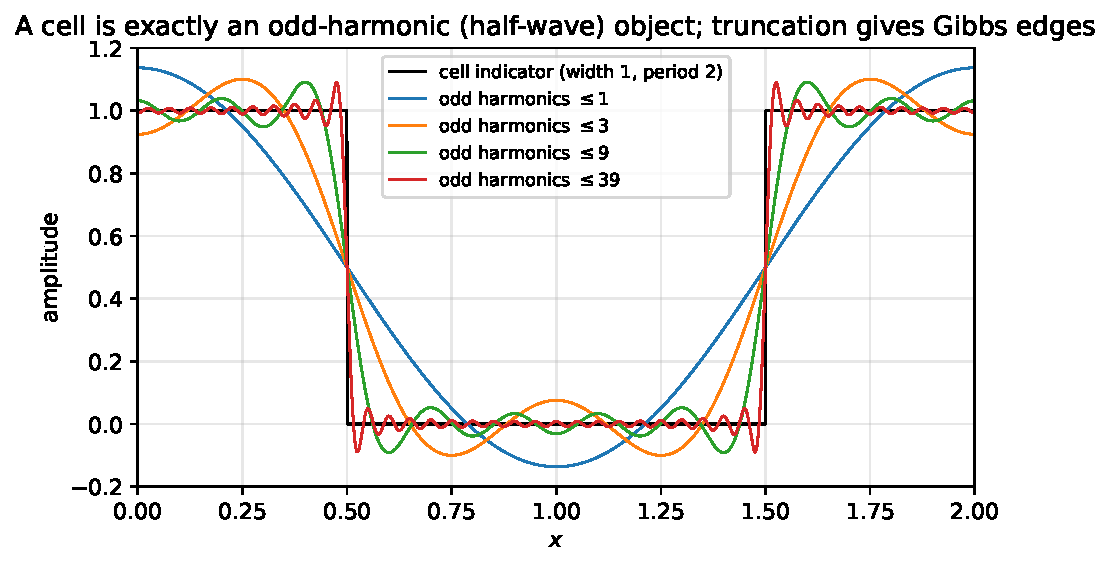
\includegraphics[keepaspectratio]{figure_paper9_1_square_wave.pdf}}
\caption{Figure 1. The cell as an exact odd-harmonic object (Gibbs
edges)}
\end{figure}

\textbf{Figure 1. The cell as a native inhabitant of the odd harmonics:
the indicator function of width 1 on period 2 (even harmonics are
exactly zero) and the Gibbs edges of odd truncated partial sums.}

\begin{center}\rule{0.5\linewidth}{0.5pt}\end{center}

\subsection{3. Half-Wavelength Censorship: Kinematic Stabilization of
Composites}\label{half-wavelength-censorship-kinematic-stabilization-of-composites}

\subsubsection{3.1 Exact bound on the anharmonic
shift}\label{exact-bound-on-the-anharmonic-shift}

The ladder on the container of a composite becomes anharmonic due to
curvature. From the identity
\((\ell+\tfrac32)^2-\ell(\ell+3)=\tfrac94\), the maximal shift is

\[
\Delta\nu_\ell=\frac{9/4}{(\ell+\tfrac32)+\sqrt{\ell(\ell+3)}},\qquad
\Delta\nu_1=\frac{9/4}{9/2}=\boxed{\tfrac12}
\]

which is exactly monotonically decreasing in \(\ell\), and \textbf{its
maximum coincides exactly with the zero point \(1/2\) at the lowest
mode} (verified in rational arithmetic). The censorship condition
``distortion shift \(\le\) half the resolution'' is satisfied not
approximately but \textbf{exactly at the limit}.

\subsubsection{3.2 Collapse time without censorship (reductio ad
absurdum)}\label{collapse-time-without-censorship-reductio-ad-absurdum}

If the shift is taken as a real dynamical phase drift, the fidelity of a
ladder with square-wave-type weights \textbf{falls below 50\% within
3--6 fundamental periods} (verified for ladders of 2--8 rungs). Just as
a classical electron falls into the nucleus in \(10^{-11}\) seconds by
continuous radiation, a composite would collapse in an instant if the
continuous channel were open.

\begin{figure}
\centering
\pandocbounded{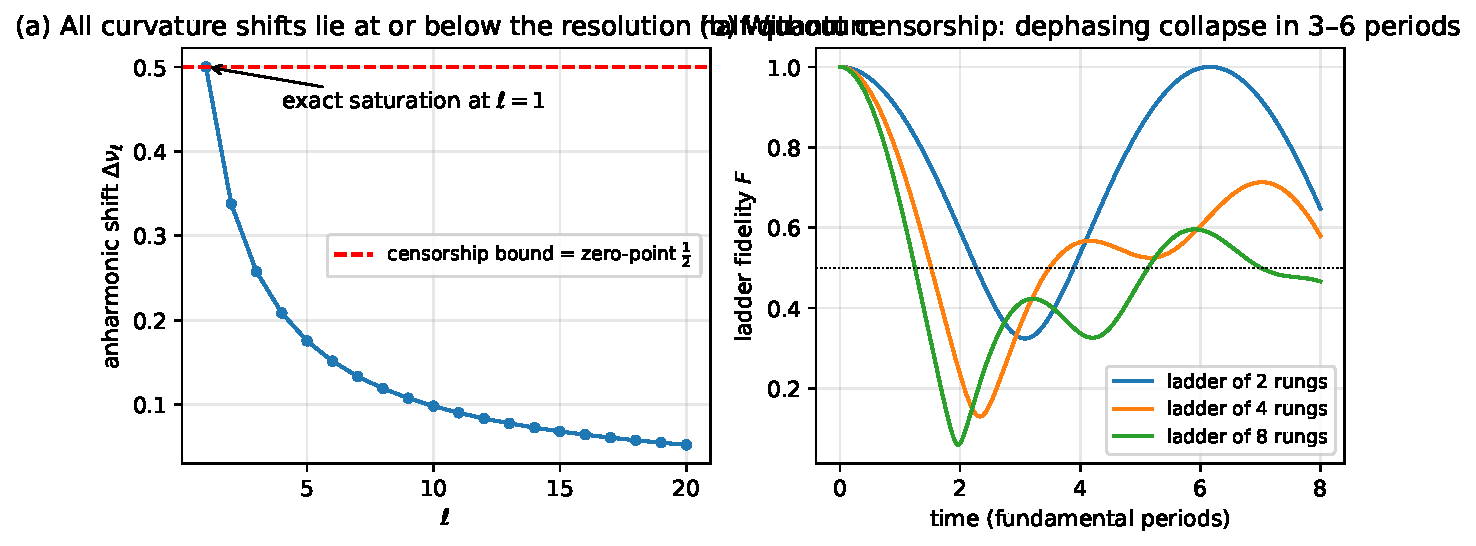
\includegraphics[keepaspectratio]{figure_paper9_2_censorship.pdf}}
\caption{Figure 2. Censorship: exact bound on anharmonic shifts and
dephasing without it}
\end{figure}

\textbf{Figure 2. (a) Exact bound on anharmonic shifts: every shift is
at most the zero point \(1/2\), with equality only at \(\ell=1\). (b)
Dephasing collapse without censorship (3--6 fundamental periods).}

\subsubsection{3.3 Stability under
censorship}\label{stability-under-censorship}

All shifts are at most half the resolution (the unit record, Paper 6
{[}3{]}), and a difference that is not recorded has no fact (the record
theorem). Therefore the continuous decay channel is
\textbf{kinematically closed}, and the only remaining decays are the
discrete channels --- coherent splitting (odd partitions + \(Z_2\) + the
capacity law, Paper 7).

{\def\LTcaptype{none} % do not increment counter
\begin{longtable}[]{@{}
  >{\raggedright\arraybackslash}p{(\linewidth - 4\tabcolsep) * \real{0.3333}}
  >{\raggedright\arraybackslash}p{(\linewidth - 4\tabcolsep) * \real{0.3333}}
  >{\raggedright\arraybackslash}p{(\linewidth - 4\tabcolsep) * \real{0.3333}}@{}}
\toprule\noalign{}
\begin{minipage}[b]{\linewidth}\raggedright
\end{minipage} & \begin{minipage}[b]{\linewidth}\raggedright
Atom (real physics)
\end{minipage} & \begin{minipage}[b]{\linewidth}\raggedright
Composite in this model
\end{minipage} \\
\midrule\noalign{}
\endhead
\bottomrule\noalign{}
\endlastfoot
Continuous decay channel & Continuous radiation of the classical
electron & Curvature dephasing (3--6 periods) \\
Quantum closing the channel & \(\hbar/2\) & \(\delta_{\min}^2=1/2\) \\
Remaining transitions & Quantum transitions between discrete spectra &
Discrete channels (enumerated in Paper 7) \\
\end{longtable}
}

The stability of composites is not a dynamical accident but a
\textbf{quantization of the deformation space} (a structural
correspondence with the Bohr model {[}7{]}; no identification is made).

\subsubsection{3.4 The cloud of the composite and the three-layer
description}\label{the-cloud-of-the-composite-and-the-three-layer-description}

From the band structure, nothing inside a composite oscillates faster
than the composite itself (the composite is its own ultraviolet cutoff).
The internal configuration is \(B_4\) gauge (Paper 6), and the
observable content is exhausted by the gauge-invariant multiplets and
the representative label (\(R=3\): cell basis 137 → multiplets 7 →
representative 1). The decay of an individual cell is gauge
non-invariant and is not defined as a physical event --- the attack
surface is far smaller than the nominal capacity.

\subsubsection{3.5 An observation concerning
dimension}\label{an-observation-concerning-dimension}

The maximal shift of the \(S^d\) ladder reduces exactly to
\(\Delta\nu_1(d)=(\sqrt d-1)^2/2\), the censorship condition \(\le1/2\)
is equivalent to \(d\in[0,4]\), and saturation occurs only at the two
endpoints. \textbf{\(d=4\) is the maximum dimension in which this
protection holds.} The status of this observation (the fixing of
normalization and coupling) is treated in Paper 11.

\begin{center}\rule{0.5\linewidth}{0.5pt}\end{center}

\subsection{4. Interference Closure Tests: The Ceiling of
Existence}\label{interference-closure-tests-the-ceiling-of-existence}

\subsubsection{4.1 Exact closure of the single
cell}\label{exact-closure-of-the-single-cell}

The indicator function of a cell of width 1 placed on period 2 makes the
even harmonics zero (to machine precision) --- width/period = 1/2 is the
\textbf{unique filling fraction} at which half-wave symmetry holds
exactly, and the cell is a native inhabitant of the odd harmonics.
Already in the minimal construction (one fundamental wave per axis), the
edge width 0.43 falls inside the zero-point width \(1/2\).

\subsubsection{4.2 The odd nesting
theorem}\label{the-odd-nesting-theorem}

The condition for the ladder of a cell (frequencies \(m/2\), \(m\) odd)
to ride on the ladder of a composite (\(n/2R\), \(n\) odd) is \(n=mR\),
that is, \textbf{the scale ratio \(R\) must be odd} (the retention rate
is 100\% for odd \(R\) and exactly 0\% for even \(R\)). The odd-\(k\)
rule of the genealogy (§2.2) is rederived from wave closure alone. A
composite with even \(R\) cannot carry a single coherent logic wavefront
--- by a route independent of the \(R^2\) classification theorem (Paper
5 {[}2{]}: single states are odd), we arrive at the same exclusion.

\subsubsection{4.3 Fundamental-wave certifiability and the three-band
structure}\label{fundamental-wave-certifiability-and-the-three-band-structure}

We judged whether a composite ``can certify its own occupancy structure
using only waves of its own wavelength,'' using the exact Fourier
coefficients of the occupancy field (structure factor × sinc, no lattice
jitter) and the eye opening in the odd bands (separation of
occupied/empty slots). The best opening under the composite-scale
criterion (wavelength of the certifying band \(\ge\) the cell fundamental
wavelength):

{\def\LTcaptype{none} % do not increment counter
\begin{longtable}[]{@{}
  >{\raggedright\arraybackslash}p{(\linewidth - 28\tabcolsep) * \real{0.0667}}
  >{\raggedright\arraybackslash}p{(\linewidth - 28\tabcolsep) * \real{0.0667}}
  >{\raggedright\arraybackslash}p{(\linewidth - 28\tabcolsep) * \real{0.0667}}
  >{\raggedright\arraybackslash}p{(\linewidth - 28\tabcolsep) * \real{0.0667}}
  >{\raggedright\arraybackslash}p{(\linewidth - 28\tabcolsep) * \real{0.0667}}
  >{\raggedright\arraybackslash}p{(\linewidth - 28\tabcolsep) * \real{0.0667}}
  >{\raggedright\arraybackslash}p{(\linewidth - 28\tabcolsep) * \real{0.0667}}
  >{\raggedright\arraybackslash}p{(\linewidth - 28\tabcolsep) * \real{0.0667}}
  >{\raggedright\arraybackslash}p{(\linewidth - 28\tabcolsep) * \real{0.0667}}
  >{\raggedright\arraybackslash}p{(\linewidth - 28\tabcolsep) * \real{0.0667}}
  >{\raggedright\arraybackslash}p{(\linewidth - 28\tabcolsep) * \real{0.0667}}
  >{\raggedright\arraybackslash}p{(\linewidth - 28\tabcolsep) * \real{0.0667}}
  >{\raggedright\arraybackslash}p{(\linewidth - 28\tabcolsep) * \real{0.0667}}
  >{\raggedright\arraybackslash}p{(\linewidth - 28\tabcolsep) * \real{0.0667}}
  >{\raggedright\arraybackslash}p{(\linewidth - 28\tabcolsep) * \real{0.0667}}@{}}
\toprule\noalign{}
\begin{minipage}[b]{\linewidth}\raggedright
\(s\)
\end{minipage} & \begin{minipage}[b]{\linewidth}\raggedright
1
\end{minipage} & \begin{minipage}[b]{\linewidth}\raggedright
3
\end{minipage} & \begin{minipage}[b]{\linewidth}\raggedright
5
\end{minipage} & \begin{minipage}[b]{\linewidth}\raggedright
7
\end{minipage} & \begin{minipage}[b]{\linewidth}\raggedright
9
\end{minipage} & \begin{minipage}[b]{\linewidth}\raggedright
11
\end{minipage} & \begin{minipage}[b]{\linewidth}\raggedright
13
\end{minipage} & \begin{minipage}[b]{\linewidth}\raggedright
17
\end{minipage} & \begin{minipage}[b]{\linewidth}\raggedright
21
\end{minipage} & \begin{minipage}[b]{\linewidth}\raggedright
25
\end{minipage} & \begin{minipage}[b]{\linewidth}\raggedright
33
\end{minipage} & \begin{minipage}[b]{\linewidth}\raggedright
49
\end{minipage} & \begin{minipage}[b]{\linewidth}\raggedright
81
\end{minipage} & \begin{minipage}[b]{\linewidth}\raggedright
121
\end{minipage} \\
\midrule\noalign{}
\endhead
\bottomrule\noalign{}
\endlastfoot
best eye & +1.64 & +0.29 & +0.23 & \textbf{\(-\)0.10} & +0.29 & +0.33 &
+0.06 & +0.12 & +0.03 & \textbf{\(-\)0.04} & \(-\)0.09 & \(-\)0.07 & \(-\)0.20 &
\(-\)0.37 \\
\end{longtable}
}

\begin{quote}
\textbf{Three-band structure}: - \textbf{Certified band
\(s\in\{1,3,5\}\)}: margin \(\ge+0.23\) with a single fundamental wave.
Coincides with the absolutely stable species of Paper 7. -
\textbf{Critical band \(s=9\)--\(21\)}: certifiable, but the margin
decays and oscillates. The exception is \(s=7\) --- the unique small
label that cannot be certified at the composite scale (coinciding with
the decay threshold). - \textbf{Forbidden band \(s\ge25\)}:
composite-scale certification disappears. For \(s\ge49\), certification
fails in \textbf{every band} of the odd sector (verified down to band
depth 31, wavelength 0.45 cells, saturating at \(-0.07\)), and the
margin deteriorates monotonically with \(s\) (\(-0.37\) at \(s=121\)).
\end{quote}

\begin{figure}
\centering
\pandocbounded{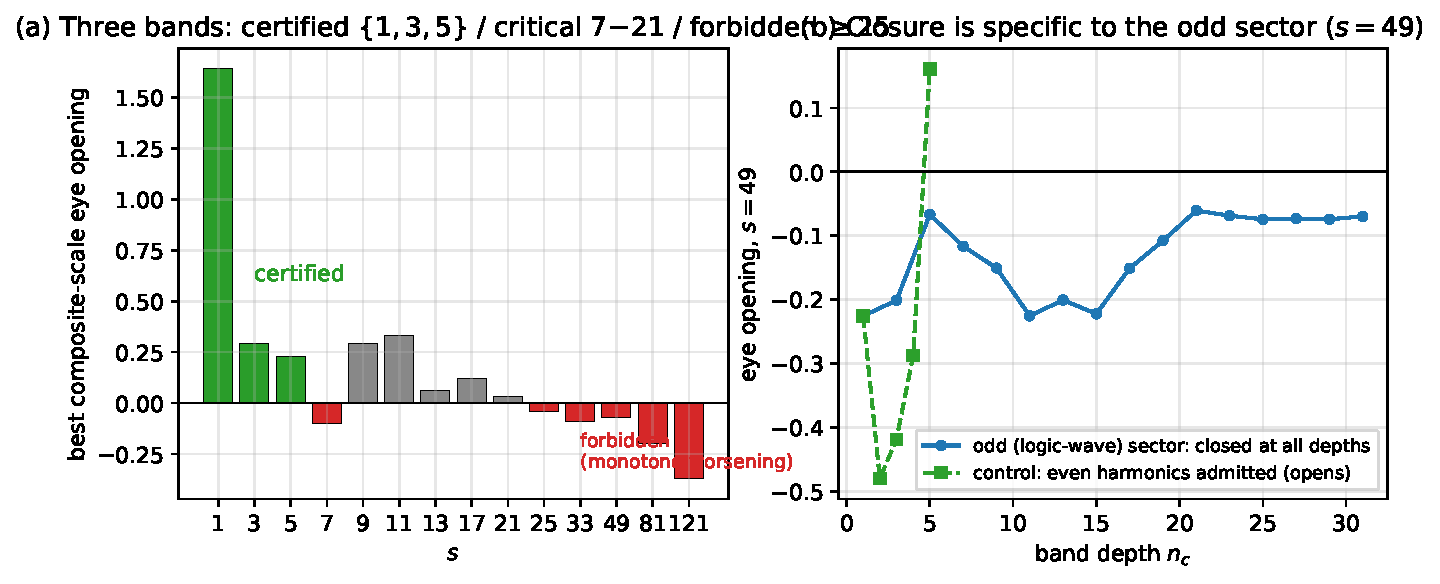
\includegraphics[keepaspectratio]{figure_paper9_3_three_bands.pdf}}
\caption{Figure 3. Three-band certification structure and odd-sector
closure}
\end{figure}

\textbf{Figure 3. (a) The three-band structure of fundamental-wave
certifiability (exact values): certified band \(\{1,3,5\}\) / critical
band / forbidden band. (b) The odd sector of \(s=49\) is closed down to
depth 31, while the control experiment (even harmonics allowed) is open
--- the closure is intrinsic to logic waves.}

\subsubsection{4.4 Control experiment: the closure is intrinsic to logic
waves}\label{control-experiment-the-closure-is-intrinsic-to-logic-waves}

In the full band with even harmonics also allowed, \(s=25\) opens at
depth 4 and \(s=49\) at depth 5. The occupancy information itself
exists, but it \textbf{can live only in the even harmonics} --- and the
even harmonics lie outside the alphabet of binary symmetric signals.
Large clusters are not ``undrawable''; they are ``\textbf{undrawable as
logic waves}.''

\subsubsection{4.5 The compulsion of
hierarchization}\label{the-compulsion-of-hierarchization}

\(s=81\) cannot exist as a single entity, but as a nesting of nine
children of \(s=9\) it can be composed entirely of entities certifiable
at every level.

\begin{quote}
A large \(S\) cannot exist as a flat cluster, but only as a nesting of
certifiable small entities. \textbf{The inward self-similar hierarchy
(Paper 4 {[}1{]}) is neither a choice nor a tendency, but a compulsion
under the logic wave ontology.} That ``clusters of high frequency cannot
exist stably'' is shown, without requiring any dynamics of decay, as a
kinematic impossibility of the mode of existence.
\end{quote}

Seen from outside, a stable species takes the form of a quasi-square
solitary wave packet that carries a built-in odd comb of spacing
\(1/R'\), is localized within an extent \(2R'\), and restores itself
every period (a minimal-uncertainty wave packet with half-width ×
fundamental wave = \(1/2\). Whereas the classical soliton {[}8{]}
cancels dispersion by nonlinearity, the wave packet of this model keeps
its shape because \textbf{censorship kills dispersion} --- a structural
correspondence).

\begin{center}\rule{0.5\linewidth}{0.5pt}\end{center}

\subsection{5. Scope of Claims of This
Paper}\label{scope-of-claims-of-this-paper}

What we claim: (1) Lattice = odd-harmonic ladder, ladder = genealogy.
(2) Absence of amplitude = coherence condition (two independent
requirements). (3) The exact bound \(1/2\) on the anharmonic shift and
kinematic stabilization by censorship (including the reductio). (4)
Exact closure of the single cell and the odd nesting theorem. (5) The
three-band structure of fundamental-wave certifiability and the
existence ceiling (\(s\ge25/49\)), the intrinsicality to logic waves
shown by the control experiment, and the compulsion of hierarchization.

What we do not claim: (1) Identification with matter, fields, or
particles in the real universe (``logic wave,'' ``stability,'' and
``wave packet'' are descriptions of modes of construction within the
model). (2) Dynamics of decay (transition rates, lifetimes). (3)
Promotion of the \(d=4\) statement (it remains an observation; the
fixing of the conditions is for Paper 11). (4) A complete description of
the longitudinal direction of the harmonic ladder (inter-level
coherence) --- the energy bookkeeping per harmonic (truncation solution
or genealogy solution) is explicitly left as an open problem.

\begin{center}\rule{0.5\linewidth}{0.5pt}\end{center}

\subsection{6. Conclusion}\label{conclusion}

The stability of composite states is supported by a two-tier structure:
the counting tier (Paper 7: the presence or absence of channels) and the
wave tier (this paper: censorship closes continuous decay, and
interference closure draws the ceiling of existence). The two are
independent computations, yet they agree on the stable species
\(\{1,3,5\}\) and the threshold \(s=7\). Moreover, the wave tier
supplied information absent from the counting --- the existence ceiling
and the compulsion of hierarchization. The mode of existence as a single
gigantic entity is, in this model, forbidden by the logic wave structure
itself.

\begin{center}\rule{0.5\linewidth}{0.5pt}\end{center}

\subsection{Appendix: Essentials of the Reproduction
Procedure}\label{appendix-essentials-of-the-reproduction-procedure}

The anharmonic shifts rest on the identity and rational arithmetic; the
collapse times on numerical integration of ladder fidelity; the closure
tests on exact Fourier coefficients (structure factor × sinc) and
exhaustive evaluation of eye openings (\(s\le121\), including robustness
checks at multiple resolutions). The scripts and research notes are
provided in the public repository
(https://github.com/WurabeSeiji/ai-chat-logs-open).

\begin{center}\rule{0.5\linewidth}{0.5pt}\end{center}

\subsection{References}\label{references}

{[}1{]} Noriaki Kihara, Paper 4, v1.0, 2026. Concept DOI:
10.5281/zenodo.20638962.

{[}2{]} Noriaki Kihara, Paper 5, v0.2, 2026. Concept DOI: 10.5281/zenodo.20640454.

{[}3{]} Noriaki Kihara, Paper 6, v0.2, 2026. Concept DOI: 10.5281/zenodo.20640456.

{[}4{]} Noriaki Kihara, Paper 7, v0.2, 2026. Concept DOI: 10.5281/zenodo.20640458.

{[}5{]} E. Hewitt and R. E. Hewitt, ``The Gibbs--Wilbraham phenomenon:
An episode in Fourier analysis,'' Archive for History of Exact Sciences
21 (1979), 129--160.

{[}6{]} C. E. Shannon, ``Communication in the presence of noise,''
Proceedings of the IRE 37 (1949), 10--21.

{[}7{]} N. Bohr, ``On the constitution of atoms and molecules,''
Philosophical Magazine 26 (1913), 1--25.

{[}8{]} N. J. Zabusky and M. D. Kruskal, ``Interaction of `solitons' in
a collisionless plasma and the recurrence of initial states,'' Physical
Review Letters 15 (1965), 240--243.

\begin{center}\rule{0.5\linewidth}{0.5pt}\end{center}

\subsection{License}\label{license}

This paper is published under CC BY 4.0.\\
Reuse, adaptation, translation, and citation are permitted, provided
that the author name, version, publication date, and source are clearly
indicated.

\end{document}
